\documentclass[11pt,a4paper,oneside,openright]{book}
\usepackage[spanish,activeacute,es-noshorthands]{babel}
\usepackage[utf8]{inputenc}
\usepackage[T1]{fontenc}
\usepackage{lmodern}
\usepackage{amsmath, amssymb, amsthm}
\usepackage{graphicx}
\graphicspath{{figuras/m13/}{figuras/}}
\usepackage[dvipsnames]{xcolor}
\usepackage{listings}
\usepackage{geometry}
\geometry{margin=2.5cm, headheight=14pt}
\usepackage{microtype}
\usepackage{booktabs}
\usepackage{longtable}
\usepackage{enumitem}
\usepackage{fancyhdr}
\usepackage{tcolorbox}
\tcbuselibrary{skins, breakable}
\usepackage{caption}
\captionsetup{font=small, labelfont=bf}
\usepackage{hyperref}
\hypersetup{
  colorlinks=true, linkcolor=NavyBlue, citecolor=ForestGreen, urlcolor=BrickRed,
  pdftitle={M13 --- Como otras misiones CubeSat open-source resolvieron lo mismo},
  pdfauthor={INTISAT --- Documentacion tecnica}
}

% ========== Estilo de cajas ==========
\definecolor{cbox-intui}{HTML}{2C5282}
\definecolor{cbox-intui-bg}{HTML}{EBF8FF}
\definecolor{cbox-warn}{HTML}{C53030}
\definecolor{cbox-warn-bg}{HTML}{FFF5F5}
\definecolor{cbox-ok}{HTML}{2F855A}
\definecolor{cbox-ok-bg}{HTML}{F0FFF4}
\definecolor{cbox-tech}{HTML}{B7791F}
\definecolor{cbox-tech-bg}{HTML}{FFFBEB}
\definecolor{cbox-payload}{HTML}{6B46C1}
\definecolor{cbox-payload-bg}{HTML}{FAF5FF}

\newtcolorbox{intui}{
  colback=cbox-intui-bg, colframe=cbox-intui, sharp corners=northwest,
  arc=2pt, boxrule=1pt, fonttitle=\bfseries,
  title=Intuicion, breakable
}
\newtcolorbox{cuidado}{
  colback=cbox-warn-bg, colframe=cbox-warn, sharp corners=northwest,
  arc=2pt, boxrule=1pt, fonttitle=\bfseries,
  title=Cuidado, breakable
}
\newtcolorbox{logrado}{
  colback=cbox-ok-bg, colframe=cbox-ok, sharp corners=northwest,
  arc=2pt, boxrule=1pt, fonttitle=\bfseries,
  title=Que adopta INTISAT, breakable
}
\newtcolorbox{tecnico}{
  colback=cbox-tech-bg, colframe=cbox-tech, sharp corners=northwest,
  arc=2pt, boxrule=1pt, fonttitle=\bfseries,
  title=Detalle tecnico, breakable
}
\newtcolorbox{payloadbox}{
  colback=cbox-payload-bg, colframe=cbox-payload, sharp corners=northwest,
  arc=2pt, boxrule=1pt, fonttitle=\bfseries,
  title=Referencias y URLs, breakable
}

\definecolor{codebg}{HTML}{F8F9FA}
\lstdefinestyle{py}{
  basicstyle=\ttfamily\footnotesize,
  backgroundcolor=\color{codebg},
  keywordstyle=\color{NavyBlue}\bfseries,
  commentstyle=\color{ForestGreen}\itshape,
  stringstyle=\color{BrickRed},
  numbers=left, numberstyle=\tiny\color{gray},
  frame=single, framerule=0.4pt, rulecolor=\color{gray},
  breaklines=true, captionpos=b, language=Python,
  showstringspaces=false, tabsize=2,
}
\lstdefinestyle{c}{
  basicstyle=\ttfamily\footnotesize,
  backgroundcolor=\color{codebg},
  keywordstyle=\color{NavyBlue}\bfseries,
  commentstyle=\color{ForestGreen}\itshape,
  stringstyle=\color{BrickRed},
  numbers=left, numberstyle=\tiny\color{gray},
  frame=single, framerule=0.4pt, rulecolor=\color{gray},
  breaklines=true, captionpos=b, language=C,
  showstringspaces=false, tabsize=2,
}

\pagestyle{fancy}
\fancyhf{}
\renewcommand{\headrulewidth}{0.4pt}
\fancyhead[L]{\small M13 --- Comparativa CubeSats open-source}
\fancyhead[R]{\small \leftmark}
\fancyfoot[C]{\thepage}
\renewcommand{\chaptermark}[1]{\markboth{#1}{}}

\title{\Huge\bfseries M13 --- Como otros lo hicieron\\[0.3em]
  \LARGE FloripaSat, OreSat, AAUSAT, UPSat y NASA\\[0.5em]
  \large Estudio comparativo de CubeSats open-source y frameworks de vuelo\\
  \normalsize Que copiar, que adaptar y que ignorar para el INTISAT}
\author{Equipo INTISAT}
\date{Mayo 2026}

\begin{document}

\frontmatter
\maketitle

\chapter*{Prefacio}

Este manual existe porque \textbf{no estamos solos}. Antes que nosotros,
varios equipos universitarios pusieron CubeSats en orbita publicando
\emph{todo} su trabajo: codigo, esquematicos, documentos de diseno, lecciones
aprendidas. Tambien la NASA libero dos de los frameworks de software de
vuelo mas usados del mundo (cFS y F'). Ignorar todo eso seria reinventar
problemas que ya fueron resueltos.

\textbf{Para que sirve este manual.} Es la respuesta sistematica a tres
preguntas que aparecen una y otra vez en las reuniones:

\begin{enumerate}[leftmargin=2em]
  \item ``Esto que estamos haciendo, $\zeta$como lo hace otra gente?''
  \item ``$\zeta$Hay un framework que ya resuelva esto y no tengamos que
    escribirlo nosotros?''
  \item ``Si la NASA usa esto en Marte, $\zeta$por que no usamos lo mismo
    nosotros?''
\end{enumerate}

\textbf{Que no es este manual.} No es un tutorial para usar cFS ni para
escribir codigo F'. Es un \emph{mapa} que muestra que existe, donde
buscarlo y, sobre todo, \emph{cuando vale la pena} usarlo y cuando
no.

\textbf{Como leerlo.} Los capitulos 1 y 2 son el marco: timeline y
matriz comparativa. Los capitulos 3 al 8 son uno por proyecto: leelos
en cualquier orden, son independientes. El capitulo 9 cierra con la
recomendacion concreta para INTISAT y la planilla de decisiones
abiertas.

\tableofcontents

\mainmatter

% ============================================================================
\chapter{Por que mirar lo que otros hicieron}
% ============================================================================

\section{La paradoja del CubeSat universitario}

Un CubeSat universitario tipico vive una paradoja: por un lado, el equipo
es chico, joven, sin experiencia previa en vuelo, con presupuesto limitado
y plazos academicos. Por el otro, debe construir un sistema embebido
distribuido, tolerante a fallas, con comunicaciones espaciales,
calificacion ambiental, software certificable y operaciones 24/7 durante
meses o anos. La unica forma honesta de cerrar esa brecha es \emph{copiar
inteligentemente}.

\begin{intui}
Copiar inteligentemente no es plagiar arquitectura completa. Es:
\begin{enumerate}[leftmargin=2em]
  \item Identificar el problema que estas resolviendo.
  \item Buscar quien lo resolvio antes en condiciones parecidas.
  \item Estudiar su solucion y sus errores documentados.
  \item Adoptar la idea, no necesariamente el codigo.
\end{enumerate}
La diferencia con plagiar es que cuando copias inteligente,
\emph{entendes} lo que copias y podes adaptarlo a tu contexto.
\end{intui}

\section{El movimiento open-source en CubeSats}

Hasta aproximadamente 2014, la mayoria de los CubeSats eran ``open'' en
nombre pero cerrados en la practica: publicaban papers academicos pero
no el codigo ni los esquematicos. La situacion cambio cuando varios
equipos universitarios empezaron a publicar TODO bajo licencias libres,
y la NASA acompano liberando sus frameworks internos. Las consecuencias
son enormes:

\begin{itemize}[leftmargin=2em]
  \item Un estudiante en cualquier universidad del mundo puede leer
    \emph{exactamente} el codigo que vola en la ISS o en Marte.
  \item Los errores quedan documentados publicamente: si una mision
    fracaso, su post-mortem suele estar online.
  \item Los protocolos se estandarizaron: CSP (Cubesat Space Protocol),
    CANopen CiA 301, ECSS-E-ST-70-41 (telemetria/telecomando), aparecen
    una y otra vez en proyectos independientes.
  \item Las herramientas se compartieron: GNU Radio, gr-satnogs y la
    red SatNOGS de estaciones terrenas distribuidas son ejemplo de
    infraestructura comun.
\end{itemize}

\section{Las 6 referencias que vamos a estudiar}

Las elegimos por dos criterios: \textbf{(a)} estar 100\% publicas (codigo
+ docs) y \textbf{(b)} representar un punto distinto del espacio de
diseno.

\begin{itemize}[leftmargin=2em]
  \item \textbf{FloripaSat (UFSC, Brasil).} El ejemplo de America Latina.
    Arquitectura \emph{distribuida}: 4 microcontroladores MSP430,
    cada uno con su propio firmware en FreeRTOS, comunicandose por SPI.
    Documentacion en LaTeX dentro del mismo repo.
  \item \textbf{OreSat (Portland State University, USA).} El ejemplo
    moderno: ``cards'' independientes sobre bus CAN con CANopen, OBC
    corriendo Linux con flight software en Python. 100\% open hardware
    y software.
  \item \textbf{AAUSAT (Aalborg University, Dinamarca).} El ejemplo
    metodologico: introdujeron el documento ``Operations Concept''
    como artefacto formal, jerarquia de modos (HSMM) y crearon el
    Cubesat Space Protocol (CSP) que hoy usan decenas de misiones.
  \item \textbf{UPSat (Libre Space Foundation, Grecia, 2017).} El
    primer CubeSat 100\% open en orbita. Modesto en alcance pero
    fundacional en filosofia.
  \item \textbf{NASA cFS (Core Flight System).} Framework modular de
    flight software de NASA Goddard. Usado en mas de 20 misiones
    incluyendo MMS, GPM, Lunar IceCube y la nave Orion de Artemis.
  \item \textbf{NASA F' (FPrime).} Framework de NASA JPL. El que volo
    en MarCO (primeros CubeSats a Marte, 2018) y en el helicoptero
    Ingenuity (72 vuelos en Marte, 2021--2024).
\end{itemize}

% ============================================================================
\chapter{Timeline y matriz comparativa}
% ============================================================================

\section{Linea de tiempo}

Para tener un marco temporal claro, conviene ver cuando lanzo cada
mision y cuando se libero cada framework.

\begin{figure}[h]
  \centering
  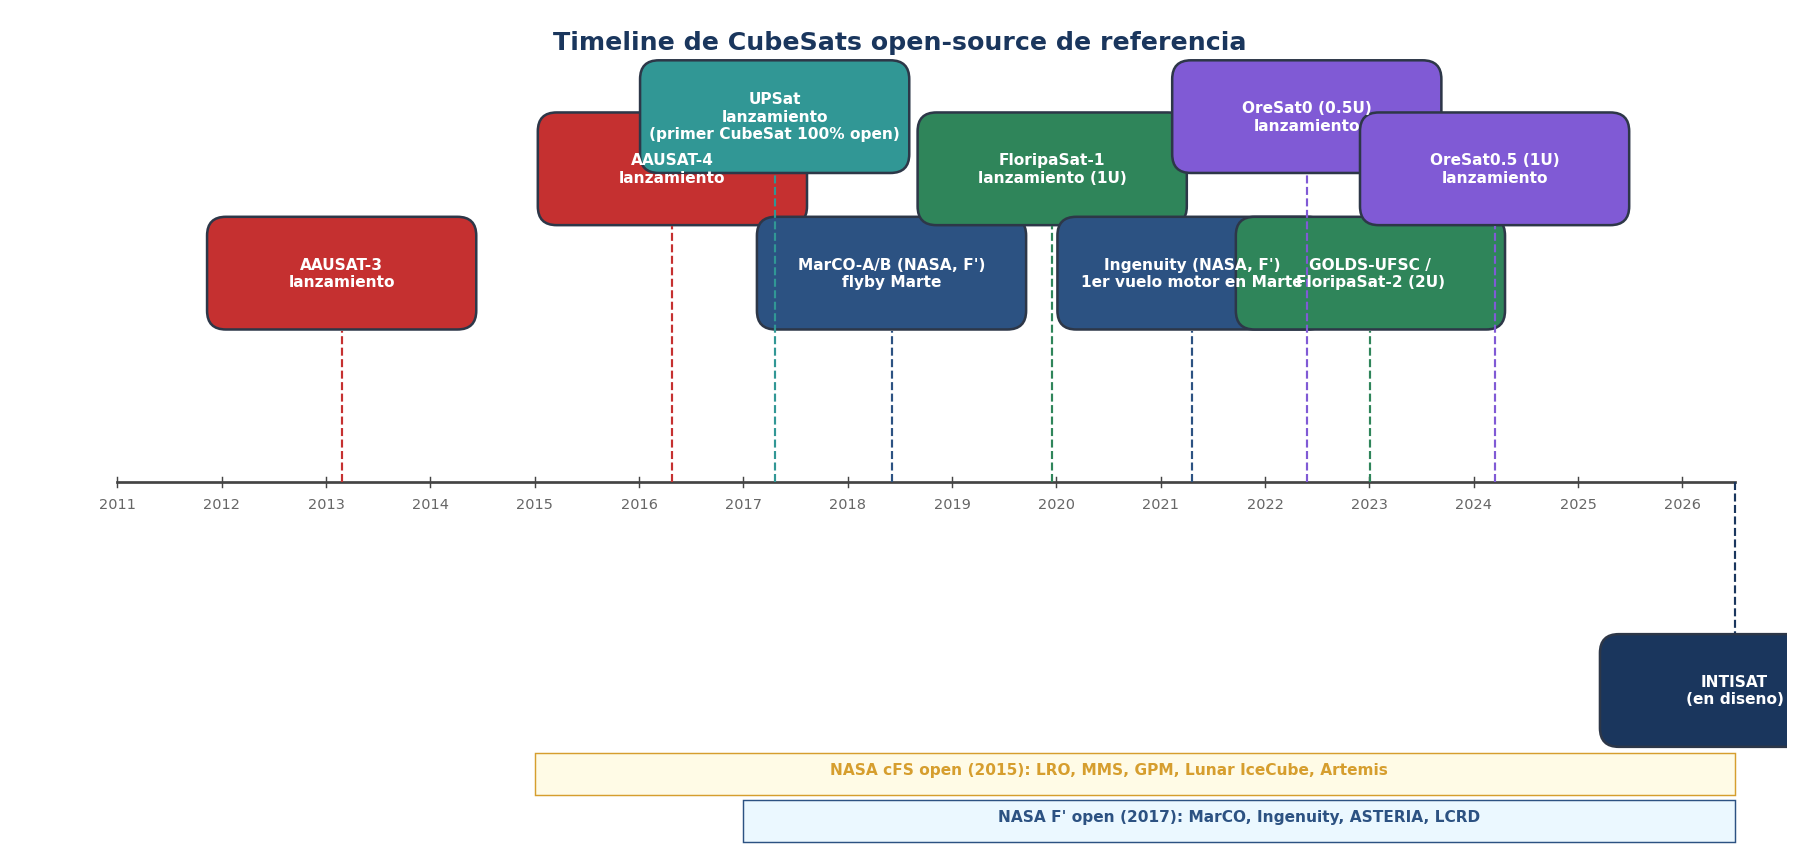
\includegraphics[width=\textwidth]{fig01_timeline.png}
  \caption{Timeline de las misiones y frameworks open-source de
  referencia. INTISAT al final, en diseno (2026).}
  \label{fig:m13-timeline}
\end{figure}

\textbf{Lectura del timeline.} AAUSAT-3 (2013) fue la primera de las
referencias academicas modernas en publicar TODO. UPSat (2017) marco
el hito ``100\% open en orbita''. Las misiones de NASA F' empezaron a
volar entre 2018 (MarCO) y 2024 (Ingenuity sigue activo), con NEA Scout,
ASTERIA y LCRD entre medio. cFS, aunque liberado en 2015, ya estaba
volando antes en versiones internas (LRO desde 2009).

\section{Matriz comparativa}

La siguiente matriz cruza los proyectos contra las 6 dimensiones que
mas nos van a importar para tomar decisiones en INTISAT: arquitectura
general, sistema operativo, bus interno, lenguaje, manejo de FSM y
licencia.

\begin{figure}[h]
  \centering
  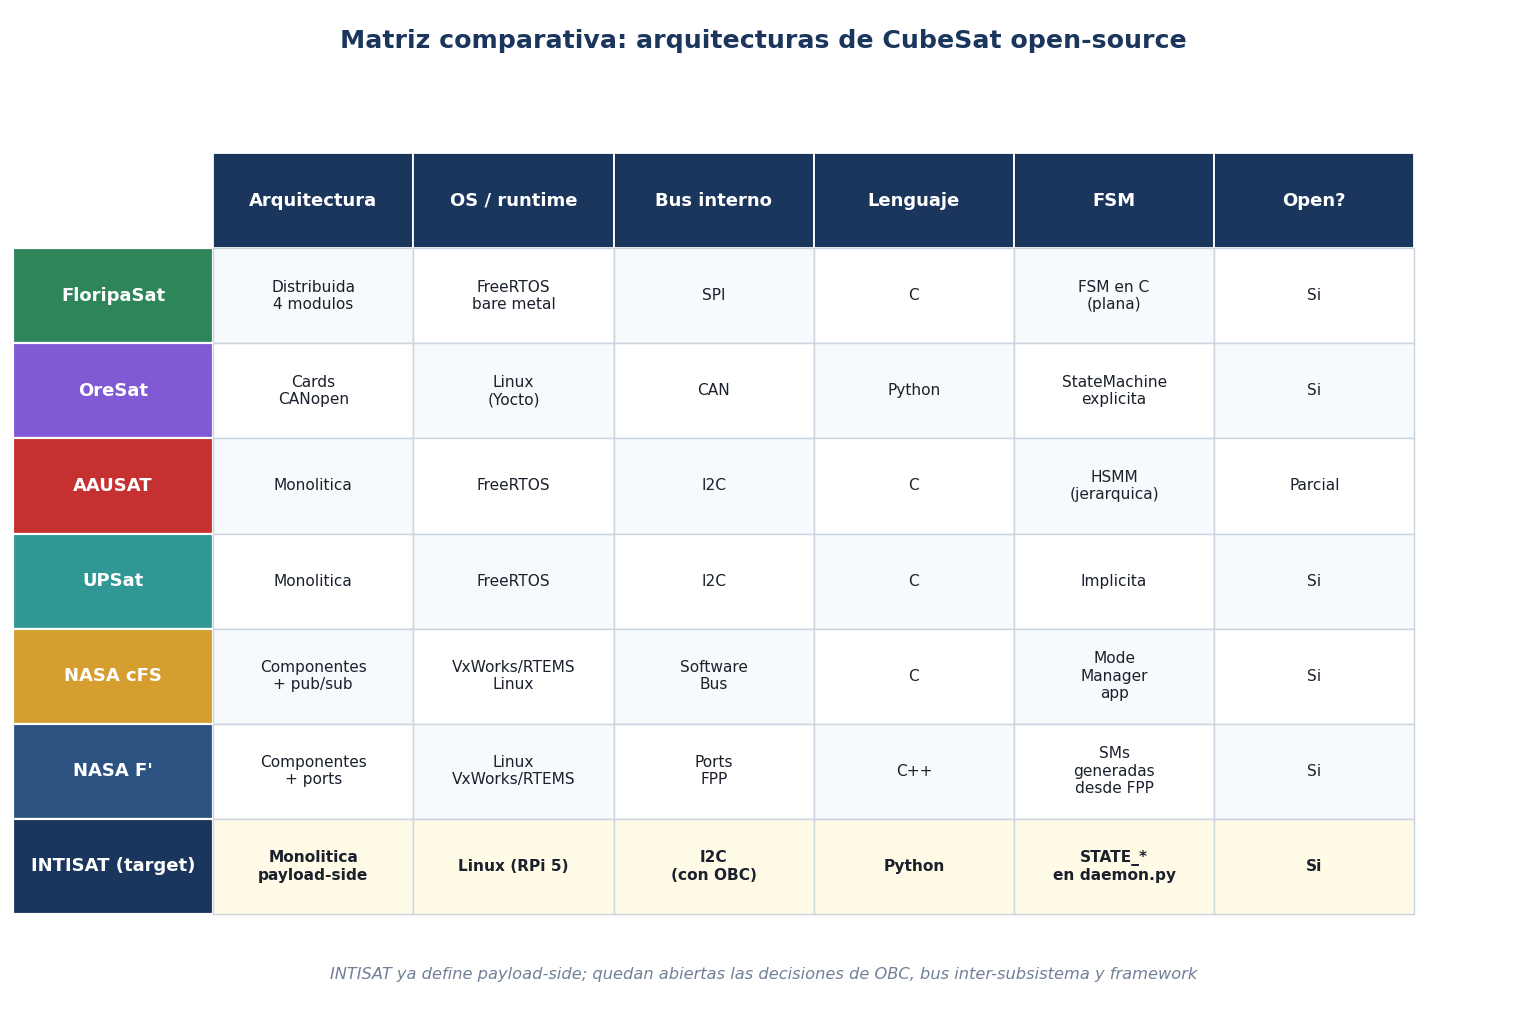
\includegraphics[width=\textwidth]{fig02_matriz.png}
  \caption{Matriz comparativa: arquitecturas y elecciones tecnicas de
  cada proyecto. La fila amarilla destaca el target del INTISAT (lo
  ya decidido del lado del payload).}
  \label{fig:m13-matriz}
\end{figure}

\begin{intui}
Notar que NO hay una sola eleccion ``correcta'' en ninguna columna.
\emph{Todas} las combinaciones que aparecen en la tabla volaron y
funcionaron. La pregunta no es ``cual es la mejor'' sino ``cual es
la mas conveniente para mi equipo, mi presupuesto, mi tiempo y mi
mision''.
\end{intui}

\textbf{Patrones que vale la pena marcar:}

\begin{itemize}[leftmargin=2em]
  \item \textbf{C domina en RTOS.} FloripaSat, AAUSAT, UPSat y cFS
    estan escritos en C corriendo sobre FreeRTOS o RTEMS/VxWorks.
    Es la combinacion clasica de software de vuelo, con cinco
    decadas de pedigri.
  \item \textbf{Python aparece donde hay Linux.} OreSat (C3 card) y
    el target del INTISAT (Raspberry Pi 5) corren Python sobre Linux.
    Esto no era posible hace 10 anos porque los OBC no tenian
    suficiente RAM. Hoy se puede.
  \item \textbf{F' usa C++} (es la excepcion). Es la apuesta de JPL
    a un lenguaje con tipos mas fuertes y generacion automatica de
    codigo desde FPP.
  \item \textbf{Tres buses distintos aparecen: SPI, I2C y CAN.}
    SPI da el throughput mas alto pero requiere chip-select por
    esclavo. I2C es lo mas barato pero menos robusto. CAN es lo
    mas robusto pero requiere transceivers en cada nodo.
\end{itemize}

\section{Como leer el resto del manual}

Los proximos 6 capitulos siguen todos la misma estructura:

\begin{enumerate}[leftmargin=2em]
  \item \textbf{El proyecto en 2 paginas.} Quien, donde, cuando.
  \item \textbf{Arquitectura.} El diagrama de bloques del sistema.
  \item \textbf{Como manejan modos / FSM.} Que aprendimos en M12.
  \item \textbf{Que adopta INTISAT y que NO.} La decision concreta.
  \item \textbf{Referencias.} URLs y papers verificables.
\end{enumerate}

Si tenes poco tiempo, podes saltar a la seccion ``Que adopta INTISAT''
de cada capitulo y leer solo eso. Pero perderias el contexto.

% ============================================================================
\chapter{FloripaSat (UFSC, Brasil)}
% ============================================================================

\section{El proyecto en 2 paginas}

\textbf{Que es.} FloripaSat es un programa de CubeSats del SpaceLab
del Departamento de Engenharia Eletronica e Eletrica de la Universidade
Federal de Santa Catarina (UFSC) en Florianopolis, Brasil. Es la
referencia mas cercana culturalmente al INTISAT: un equipo
universitario de un pais latinoamericano que decidio publicar TODO
y documentarlo en LaTeX.

\textbf{Misiones.}
\begin{itemize}[leftmargin=2em]
  \item \textbf{FloripaSat-1} (1U, 1 kg). Lanzado el 20 de diciembre
    de 2019 desde el Centro de Lanzamiento de Taiyuan (China), en un
    cohete Long March 4B (CZ-4B) como secundario de la mision
    CBERS-04A. Sigue operativo a la fecha de este manual. Mision:
    demostracion tecnologica de subsistemas open-source y radio
    amateur.
  \item \textbf{FloripaSat-2 / GOLDS-UFSC} (2U). Lanzado en enero de
    2023 en el SpaceX Transporter-6. Continuacion con payload
    cientifico de medicion de electrojet ecuatorial.
\end{itemize}

\textbf{Filosofia.} Cada subsistema del CubeSat es un repositorio de
GitHub independiente, con su propio hardware, firmware y documentacion
en LaTeX. La comunicacion entre subsistemas es por SPI. El equipo
publico una serie de papers en conferencias LARS, IAA y SBC-WSAC con
detalles tecnicos.

\textbf{Lenguaje.} Todo en C, sin ningun Python en orbita. El
microcontrolador es MSP430 de Texas Instruments.

\section{Arquitectura distribuida}

\begin{figure}[h]
  \centering
  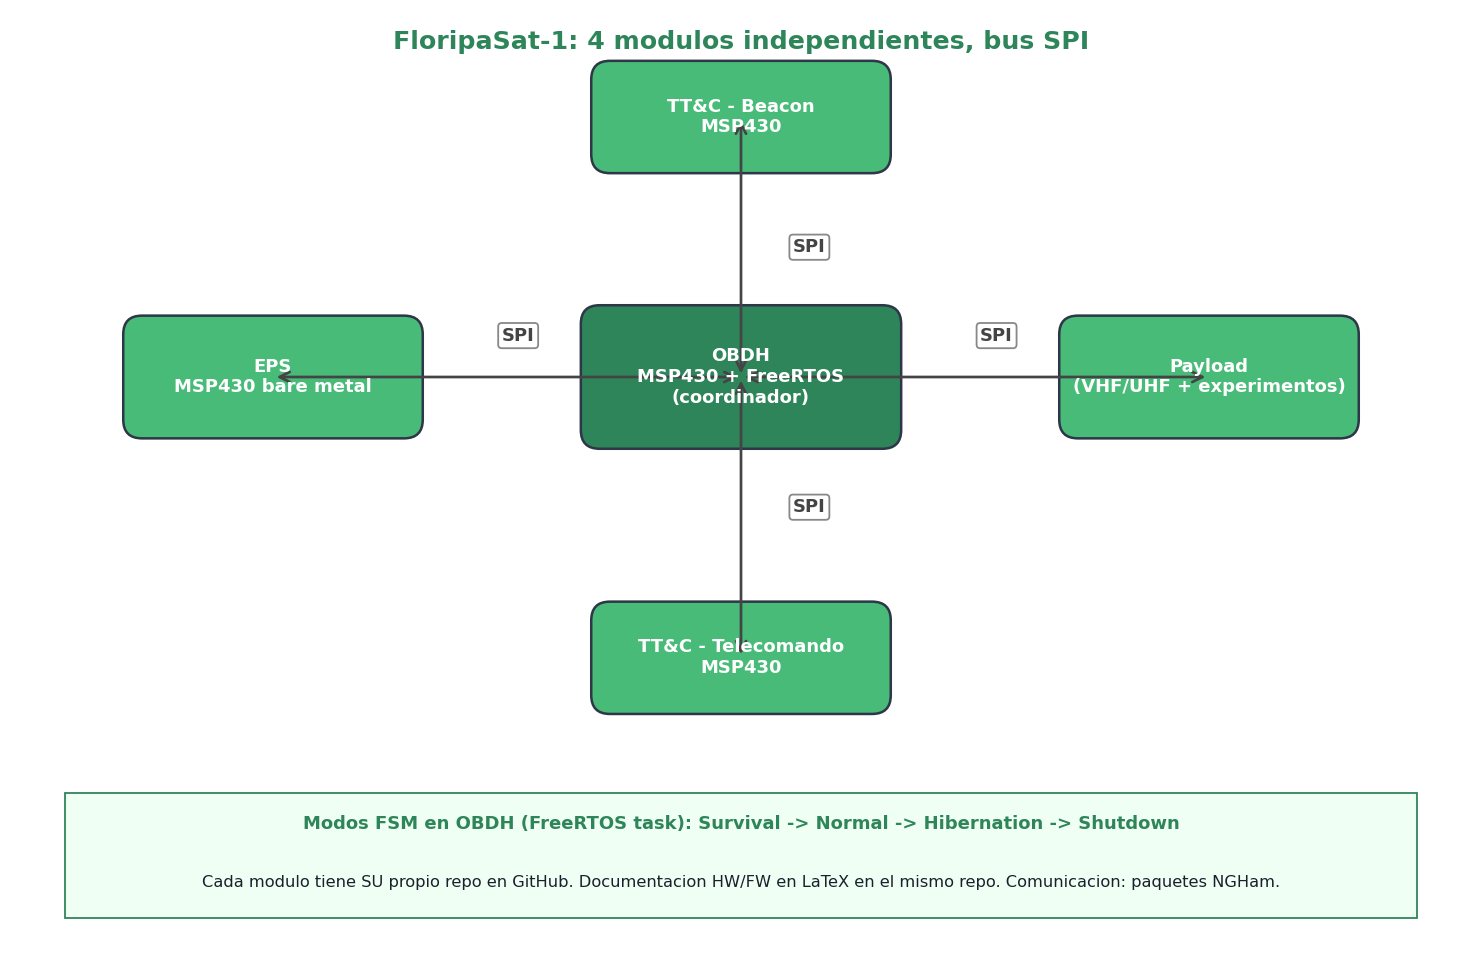
\includegraphics[width=\textwidth]{fig03_floripasat.png}
  \caption{Arquitectura de FloripaSat-1: 4 modulos independientes
  alrededor del OBDH (On-Board Data Handling), comunicandose por SPI.
  Cada modulo tiene su propio MSP430 y su propio repositorio.}
  \label{fig:m13-floripasat}
\end{figure}

Los 4 modulos son:

\begin{enumerate}[leftmargin=2em]
  \item \textbf{OBDH (On-Board Data Handling).} El cerebro coordinador.
    MSP430 corriendo FreeRTOS. Mantiene el reloj, la FSM de modos
    operacionales, la telemetria global y la cola de telecomandos.
  \item \textbf{EPS (Electrical Power System).} Otro MSP430, esta vez
    \emph{bare metal} (sin RTOS) porque su tarea es muy acotada:
    leer ADCs de las celdas solares y baterias, controlar MPPT,
    apagar lineas de alimentacion cuando hay sobrecorriente.
  \item \textbf{TT\&C Beacon.} Transmisor automatico que cada cierto
    tiempo manda un paquete de telemetria basica en VHF para que
    estaciones de radio amateur de todo el mundo lo puedan recibir.
  \item \textbf{TT\&C Telecomando.} Receptor UHF que escucha
    comandos enviados desde la estacion terrena de UFSC.
\end{enumerate}

\begin{tecnico}
\textbf{Por que cuatro micros y no uno solo.} La razon es \emph{tolerancia
a fallas}. Si el OBDH se cuelga, el EPS sigue gestionando la energia y
el Beacon sigue transmitiendo. El equipo de UFSC cita esta tolerancia
como la principal razon de la arquitectura distribuida. La contra es
que ahora tenes 4 firmwares que mantener en lugar de uno.
\end{tecnico}

\section{Como manejan modos / FSM}

FloripaSat-1 define 4 modos operacionales que viven en una FSM dentro
del OBDH (FreeRTOS task dedicada):

\begin{itemize}[leftmargin=2em]
  \item \textbf{Survival.} Modo inicial post-deploy. Solo radio
    activa, todo lo demas apagado. Espera ventana de tierra.
  \item \textbf{Normal.} Operacion estandar: telemetria, beacon,
    payload activo si la energia alcanza.
  \item \textbf{Hibernation.} Modo bajo consumo cuando bateria baja
    de un umbral. Apaga payload, deja solo housekeeping minimo.
  \item \textbf{Shutdown.} Critico: bateria muy baja, apaga TODO menos
    el watchdog que espera carga solar.
\end{itemize}

Esto se mapea casi 1-a-1 a los modos que ya defini\'o el equipo INTISAT
en el manual M12 (BOOT/SAFE/STANDBY/CAPTURA/COMM/CRITICAL). La FSM esta
implementada como un \texttt{switch} clasico en C, sin librerias de
state machines.

\section{Que adopta INTISAT y que no}

\begin{logrado}
\textbf{Adoptamos:}
\begin{itemize}[leftmargin=2em]
  \item \textbf{Repositorio por subsistema} con su propia documentacion
    en LaTeX. Ya lo estamos haciendo (este manual es ejemplo).
  \item \textbf{FSM de modos en una task dedicada} del OBDH.
  \item \textbf{Beacon independiente del OBDH.} Es radio
    amateur-friendly y nos da un canal de telemetria minima incluso
    si el OBDH falla.
\end{itemize}

\textbf{NO adoptamos:}
\begin{itemize}[leftmargin=2em]
  \item \textbf{4 microcontroladores fisicos.} Nuestro presupuesto
    de masa y energia favorece una OBC unica (Raspberry Pi CM5)
    con cosubsistemas (EPS, ADCS) atendidos por micros muy chicos.
  \item \textbf{C bare metal.} Vamos a Python sobre Linux donde
    podamos porque acelera desarrollo 5-10$\times$ y nuestro
    equipo tiene mas experiencia ahi.
\end{itemize}
\end{logrado}

\section{Referencias}

\begin{payloadbox}
\textbf{Web oficial.} \url{https://floripasat.ufsc.br/}\\[0.3em]
\textbf{Organizacion en GitHub.} \url{https://github.com/floripasat}\\[0.3em]
\textbf{Repositorios principales.}
\begin{itemize}[leftmargin=2em]
  \item \texttt{floripasat/obdh} --- firmware del OBDH
  \item \texttt{floripasat/eps} --- firmware del EPS
  \item \texttt{floripasat/ttc} --- firmware del transceptor
  \item \texttt{floripasat/payloads-x} --- payloads cientificos
  \item \texttt{floripasat/manual} --- documentacion en LaTeX
\end{itemize}
\textbf{Paper de referencia.} Marcelino et al., ``FloripaSat-1:
Lessons Learned from a Brazilian Open Source CubeSat Mission'',
publicado en SBESC/WSCAD/LARS (consultar el repo principal para
versiones actualizadas).
\end{payloadbox}

% ============================================================================
\chapter{OreSat (Portland State University, USA)}
% ============================================================================

\section{El proyecto en 2 paginas}

\textbf{Que es.} OreSat es el programa de CubeSats del Portland State
Aerospace Society (PSAS), de Portland State University, Oregon. Es
probablemente el CubeSat universitario \emph{mas modernamente
construido} de las referencias: pensado desde el dia uno como un
producto open hardware industrial-grade, con bus CANopen, OBC
corriendo Linux y flight software en Python.

\textbf{Misiones.}
\begin{itemize}[leftmargin=2em]
  \item \textbf{OreSat0} (0.5U). Lanzado el 12 de septiembre de 2022
    desde Kodiak (Alaska) en el cohete Astra LV0009. La mision
    primaria fue demostrar el bus de cards. Operaciones limitadas
    por anomalia del lanzador.
  \item \textbf{OreSat0.5} (1U). Lanzado en marzo de 2024 en el
    SpaceX Transporter-10 desde Vandenberg. Misma arquitectura,
    forma factor mayor, ahora con experimentos cientificos.
  \item \textbf{OreSat-1} (3U). En desarrollo a la fecha de este
    manual.
\end{itemize}

\textbf{Filosofia.} ``Cards'' independientes que se conectan por bus
CAN, hablando CANopen (estandar industrial CiA 301). Cada card es
un STM32 con su propio Object Dictionary. La excepcion es la \textbf{C3
card}, que corre Linux con un demonio en Python llamado OLAF
(\emph{OreSat Linux App Framework}) y actua como CANopen master.

\textbf{Lenguaje.} Python (OLAF, Linux) para la C3. C bare metal
(STM32) para el resto de cards.

\section{La arquitectura ``cards'' sobre bus CAN}

\begin{figure}[h]
  \centering
  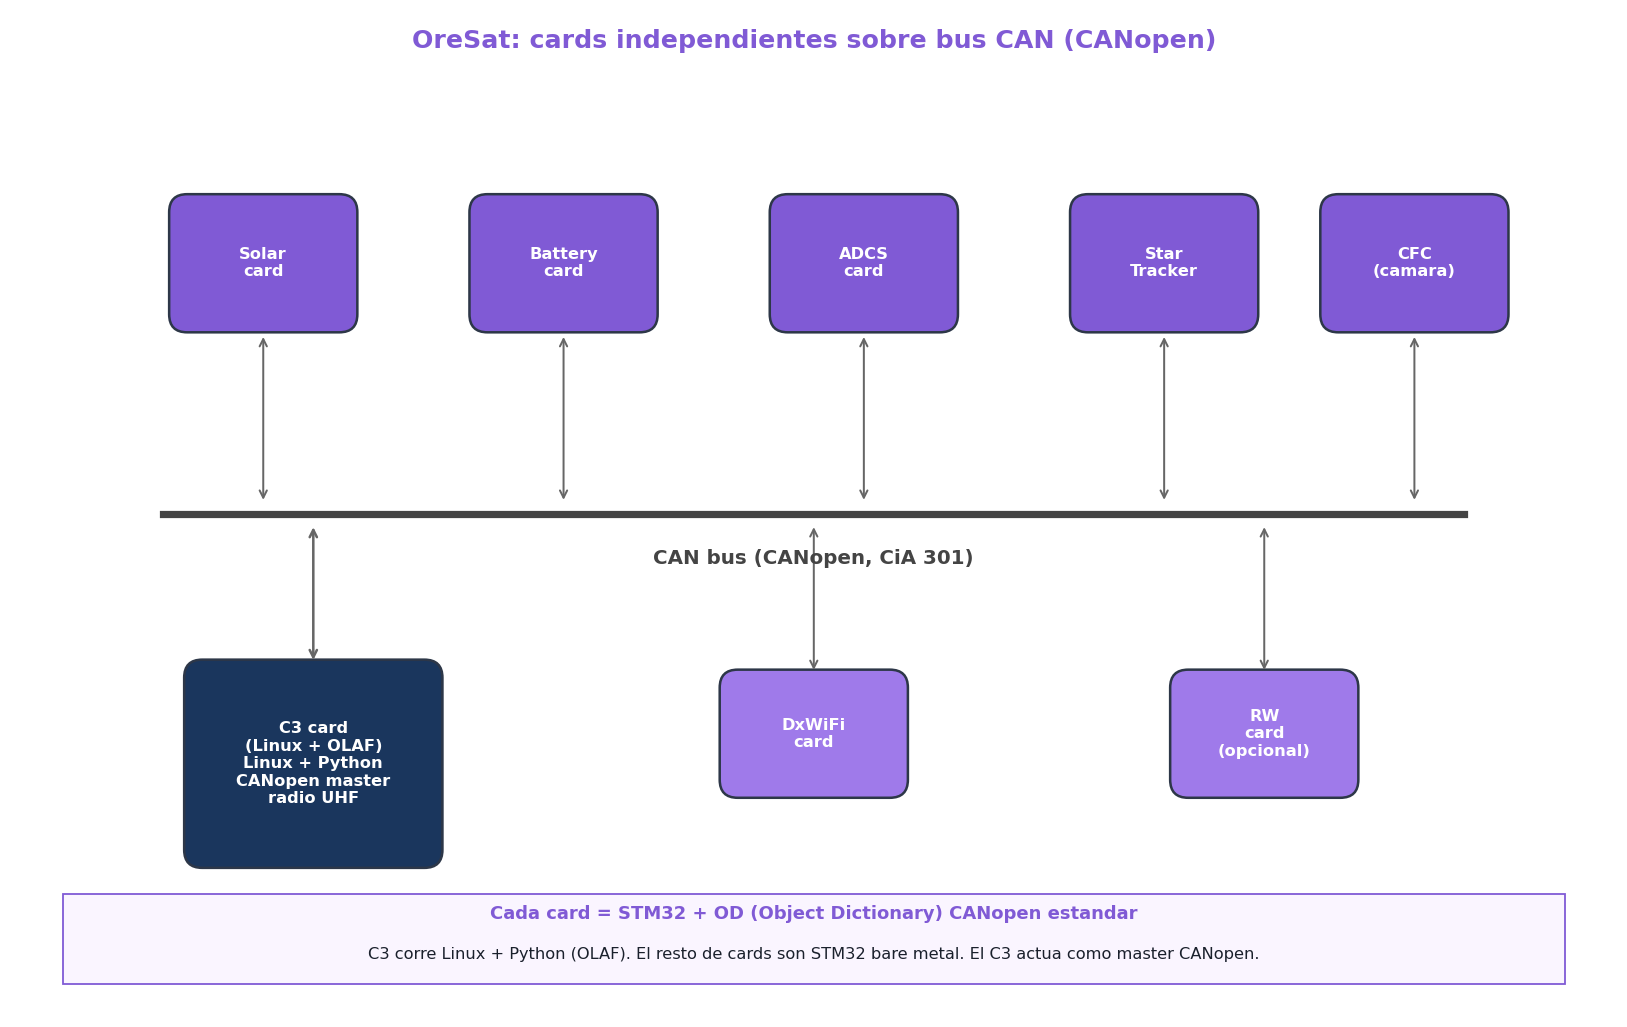
\includegraphics[width=\textwidth]{fig04_oresat.png}
  \caption{OreSat: cada subsistema es una ``card'' que se conecta al
  backplane CAN. La C3 card es el cerebro Linux. Las demas son STM32
  CANopen-compliant.}
  \label{fig:m13-oresat}
\end{figure}

\begin{tecnico}
\textbf{Que es un Object Dictionary en CANopen.} Cada nodo CANopen
expone una tabla de objetos indexada por (index, subindex) de 16+8
bits. Cada objeto puede ser leido o escrito por otro nodo enviando
un \emph{SDO} (Service Data Object), o publicarse periodicamente como
un \emph{PDO} (Process Data Object). En la practica: cada card de
OreSat \emph{declara} su telemetria y sus parametros en un archivo
EDS (Electronic Data Sheet), y la C3 los lee con un nombre estable
sin necesidad de saber detalles del firmware de la card. Es
analogo a un ROS topic, pero a nivel de hardware.
\end{tecnico}

\textbf{Que cards existen.}

\begin{itemize}[leftmargin=2em]
  \item \textbf{C3 card.} Octavo Industries OSD3358-SM (TI Sitara
    ARM Cortex-A8 + microcontrolador PRU + DSP). Corre Debian Linux.
    Es el cerebro: maneja telecomando UHF, telemetria descendente,
    coordina las otras cards.
  \item \textbf{Battery card.} STM32 que gestiona el banco de
    baterias y reporta carga al CAN.
  \item \textbf{Solar card.} STM32 que mide cada panel solar y
    reporta corriente.
  \item \textbf{ADCS card.} STM32 con magnetorquers para apuntamiento.
  \item \textbf{Star Tracker.} OreSat publico ademas su propio star
    tracker hecho de una camara industrial + ARM.
  \item \textbf{CFC (Cirrus Flux Camera).} Camara cientifica para
    medir flujo de radiacion.
  \item \textbf{DxWiFi.} Card experimental para comunicar a alta
    velocidad cuando el satelite pasa sobre la estacion terrena.
\end{itemize}

\section{Como manejan modos / FSM}

La C3 card es la que mantiene la maquina de estados global. Estados
documentados:

\begin{itemize}[leftmargin=2em]
  \item \texttt{PRE\_DEPLOY} --- timer de 30 minutos post-eyeccion.
  \item \texttt{DEPLOY} --- despliegue de antenas.
  \item \texttt{STANDBY} --- normal, beaconing.
  \item \texttt{BEACON} --- transmision activa al pasar sobre
    estacion.
  \item \texttt{EDL} --- Engineering / Diagnostics Link.
  \item \texttt{SAFE} --- modo de baja energia.
\end{itemize}

OLAF implementa la FSM en Python con clases explicitas y un dispatcher
de eventos. Cada card tiene ademas su propia mini-FSM de salud (NMT
Node State de CANopen: Initialization, Pre-Operational, Operational,
Stopped) que es estandar de CANopen, no algo inventado por OreSat.

\section{Que adopta INTISAT y que no}

\begin{logrado}
\textbf{Adoptamos:}
\begin{itemize}[leftmargin=2em]
  \item \textbf{Linux + Python en el OBC.} Misma eleccion: nuestro
    equivalente del C3 es el Raspberry Pi CM5.
  \item \textbf{Object Dictionary explicito (concepto).} Para
    INTISAT no llegamos a usar CANopen, pero la idea de \emph{declarar}
    en un archivo de texto la telemetria que expone cada subsistema
    nos sirve para definir la API I2C de manera disciplinada.
  \item \textbf{Modo \texttt{PRE\_DEPLOY} con timer obligatorio.} Es
    requisito del proveedor de lanzamiento para no encender
    transmisores antes de separarse del cohete.
\end{itemize}

\textbf{NO adoptamos:}
\begin{itemize}[leftmargin=2em]
  \item \textbf{Bus CAN.} INTISAT 1U va a usar I2C para reducir BOM,
    masa y consumo. CAN seria sobre-ingenieria para 3 subsistemas.
  \item \textbf{Una card fisica por subsistema.} INTISAT integra
    OBC + payload en la misma CM5; EPS y ADCS son perifericos I2C
    de la CM5.
\end{itemize}
\end{logrado}

\section{Referencias}

\begin{payloadbox}
\textbf{Web oficial.} \url{https://www.oresat.org/}\\[0.3em]
\textbf{Organizacion en GitHub.} \url{https://github.com/oresat}\\[0.3em]
\textbf{Repos clave.}
\begin{itemize}[leftmargin=2em]
  \item \texttt{oresat/oresat-c3} --- firmware Linux + OLAF
  \item \texttt{oresat/oresat-olaf} --- framework Python OLAF
  \item \texttt{oresat/oresat-configs} --- Object Dictionaries
    de todas las cards
\end{itemize}
\textbf{Standards.} CANopen CiA 301 (Cabezada del CAN in Automation),
disponible en \url{https://www.can-cia.org/can-knowledge/canopen/}.
\end{payloadbox}

% ============================================================================
\chapter{AAUSAT (Aalborg University, Dinamarca)}
% ============================================================================

\section{El proyecto en 2 paginas}

\textbf{Que es.} El programa AAUSAT de la Aalborg University es uno
de los pioneros mundiales en CubeSats universitarios (desde el inicio
de los 2000), y es probablemente el mas \emph{metodologicamente
riguroso} de la lista. Su contribucion mayor no es un satelite
puntual: es un conjunto de \emph{artefactos de ingenieria} que el
resto del mundo CubeSat adopto.

\textbf{Misiones.}
\begin{itemize}[leftmargin=2em]
  \item \textbf{AAUSAT-3} (1U). Lanzado 25 de febrero de 2013 desde
    Sriharikota (India) en el PSLV-C20. Demostro AIS (Automatic
    Identification System) marino desde orbita.
  \item \textbf{AAUSAT-4} (1U). Lanzado el 25 de abril de 2016 en
    el Soyuz Sentinel-1B.
  \item Tambien AAUSAT-1 (2003) y AAUSAT-II (2008) anteriores.
\end{itemize}

\textbf{Filosofia.} AAUSAT NO es el satelite mas elegante. Su valor
esta en \emph{como se documenta y se decide}. Tres aportes
fundamentales:

\begin{enumerate}[leftmargin=2em]
  \item \textbf{El documento ``Operations Concept''}, que define
    \emph{antes} de codear, todos los modos operacionales, sus
    transiciones, las ventanas de tiempo en cada modo y el
    comportamiento esperado del sistema.
  \item \textbf{HSMM (Hierarchical State Machine Model)} --- los modos
    no son una lista plana, sino una jerarquia donde ``Normal'' es
    padre de varios sub-modos. Esto es el patron \emph{statechart}
    de Harel.
  \item \textbf{CSP (Cubesat Space Protocol).} Un protocolo de red
    inspirado en TCP/IP pero adaptado a links espaciales. Se libero
    como \texttt{libcsp} (C, MIT) y hoy lo usan decenas de misiones
    (incluido GomSpace, que es spin-off de la universidad).
\end{enumerate}

\textbf{Lenguaje.} C sobre FreeRTOS para todos los modulos.

\section{Arquitectura monolitica + CSP}

A nivel hardware, AAUSAT-3/4 son monoliticos: una OBC central conectada
por I2C a EPS, ADCS y radio. Lo interesante no es el cableado, es la
\emph{capa de red}: arriba de I2C corre CSP, que abstrae el bus fisico
como si fuera una red IP.

\begin{tecnico}
\textbf{CSP en una linea.} CSP es a un CubeSat lo que TCP/IP es a
Internet: una capa de transporte con direcciones de nodo (5 bits),
puertos (6 bits), routing por hops y soporte para encriptacion HMAC.
Tu codigo NO sabe si el destino esta detras de I2C, CAN o radio: solo
manda un paquete a \texttt{(node=2, port=10)} y CSP se encarga.

\textbf{Por que importa.} Te permite mover un subsistema del bus
interno al downlink sin cambiar el codigo de aplicacion. Y te permite
hacer testeo en tierra con un nodo CSP corriendo en una laptop como
si fuera un subsistema del satelite.
\end{tecnico}

\section{Como manejan modos / FSM (HSMM)}

Aqui esta la contribucion teorica fuerte. AAUSAT estructura los modos
como una \emph{jerarquia}, no una lista:

\begin{itemize}[leftmargin=2em]
  \item \textbf{Detumbling} (modo padre, post-deploy)
  \item \textbf{Safe Mode} (modo padre)
    \begin{itemize}
      \item Beacon ON
      \item Beacon OFF (silencio total para reducir consumo)
    \end{itemize}
  \item \textbf{Normal Mode} (modo padre)
    \begin{itemize}
      \item Pointing
      \item Payload acquisition
      \item Downlink
    \end{itemize}
\end{itemize}

\textbf{Por que jerarquica.} Las transiciones de SEGURIDAD (e.g.,
``bateria $<$ 30\%'') aplican a TODOS los sub-modos del padre. Lo
escribis una vez en el padre, no en cada hoja. Es exactamente la
ventaja de los \emph{statecharts} de Harel sobre las FSM planas.

\section{Que adopta INTISAT y que no}

\begin{logrado}
\textbf{Adoptamos:}
\begin{itemize}[leftmargin=2em]
  \item \textbf{Documento ``Operations Concept'' antes de codear.}
    El manual M12 cumple ese rol: define todos los modos, transiciones
    y comportamientos ANTES de que se escriba la primera linea de
    \texttt{intisat\_payload\_daemon.py} final.
  \item \textbf{Pensar los modos como jerarquia.} Aun si la
    implementacion en INTISAT es plana al inicio, mentalmente
    diferenciamos modos ``operacionales'' de modos ``de seguridad''
    porque las transiciones tienen prioridades distintas.
\end{itemize}

\textbf{Pendiente de evaluar:}
\begin{itemize}[leftmargin=2em]
  \item \textbf{Usar libcsp en INTISAT.} Es C portable, esta empaquetado
    para Linux y FreeRTOS, y nos daria capa de red sobre I2C. Habria
    que verificar si conviene la complejidad para una mision 1U.
\end{itemize}
\end{logrado}

\section{Referencias}

\begin{payloadbox}
\textbf{Web del grupo.}
\url{https://www.space.aau.dk/cubesat/}\\[0.3em]
\textbf{libcsp en GitHub.}
\url{https://github.com/libcsp/libcsp}\\[0.3em]
\textbf{Documento ``Operations Concept''.} Buscar como
``AAUSAT Operations Concept'' en los reports tecnicos del grupo. El
formato fue replicado por varios CubeSats europeos posteriores.\\[0.3em]
\textbf{Paper canonical.} ``CubeSat Communication System, a New Open
Source Design'' --- Aalborg University.
\end{payloadbox}

% ============================================================================
\chapter{UPSat (Libre Space Foundation, Grecia)}
% ============================================================================

\section{El proyecto en 2 paginas}

\textbf{Que es.} UPSat es el primer CubeSat en orbita que es 100\%
open source: tanto el hardware (esquematicos, gerbers, BOM) como el
software (firmware, ground station, protocolo de tierra). Fue
desarrollado por la Universidad de Patras junto con la Libre Space
Foundation (ONG sin fines de lucro con sede en Atenas) como parte de
la mision QB50.

\textbf{Mision.}
\begin{itemize}[leftmargin=2em]
  \item \textbf{UPSat} (2U). Lanzado el 18 de abril de 2017 desde Cabo
    Canaveral en el SpaceX CRS-11 hacia la ISS, y eyectado desde el
    NanoRacks deployer de la ISS poco despues. Mision: medicion de
    composicion de la termosfera (sensor INMS).
\end{itemize}

\textbf{Filosofia.} La declaracion de la Libre Space Foundation es
clara: ``el espacio es un commons y la unica forma de democratizarlo
es publicar TODO''. UPSat es la prueba de concepto. Tambien
desarrollaron la red SatNOGS (estaciones terrenas distribuidas) y
herramientas como gr-satnogs (bloques GNU Radio).

\textbf{Lenguaje.} C sobre FreeRTOS, microcontroladores STM32.

\section{Arquitectura}

UPSat es monolitica: una OBC STM32 conectada por I2C a EPS, ADCS y
radio (modulo CC1101). El payload es un INMS (Ion-Neutral Mass
Spectrometer) externo. El bus interno es I2C, sin CSP ni CANopen.

\textbf{Lo importante de UPSat es el PROCESO, no la arquitectura.} El
proyecto fue ejecutado con metodologias de ingenieria espacial reales
(ECSS adaptado), con un Wiki publico donde el equipo registraba sus
decisiones y problemas. Eso es la lec\-cion mas reusable.

\section{Como manejan modos / FSM}

UPSat no documento una FSM explicita tan rica como AAUSAT. Los modos
son: \texttt{DEPLOYMENT}, \texttt{NOMINAL}, \texttt{SAFE} y
\texttt{EMERGENCY}, definidos en el firmware del OBC como
\texttt{enum} en C. Las transiciones estan implementadas implicitamente
como \texttt{if/else} dentro del main loop. Es la version mas simple
posible de FSM y aun asi resulto suficiente para operar el satelite
durante meses.

\begin{intui}
La leccion de UPSat es que \textbf{no necesitas un framework de FSM
fancy para volar un CubeSat 1U/2U}. Un \texttt{switch} en C con 4 modos
es suficiente. Lo que importa es:
\begin{enumerate}[leftmargin=2em]
  \item Documentar los modos en un papel ANTES.
  \item Que esten codificados en una sola funcion identificable.
  \item Que esten testeados en tierra.
\end{enumerate}
\end{intui}

\section{Que adopta INTISAT y que no}

\begin{logrado}
\textbf{Adoptamos:}
\begin{itemize}[leftmargin=2em]
  \item \textbf{Organizacion en GitHub publica con Wiki.} Es nuestro
    modelo de gobernanza.
  \item \textbf{Aceptar que 4-6 modos en una FSM plana es suficiente.}
    No vamos a sobre-disenar.
  \item \textbf{Usar ECSS adaptado para telemetria y telecomando.}
    Paquetes con header de servicio (ECSS-E-ST-70-41).
\end{itemize}

\textbf{NO adoptamos:}
\begin{itemize}[leftmargin=2em]
  \item \textbf{STM32 + C.} Nuestra OBC es Raspberry Pi CM5 + Python.
    UPSat representa el approach ``minimal C'' que NO es el nuestro.
\end{itemize}
\end{logrado}

\section{Referencias}

\begin{payloadbox}
\textbf{Web de Libre Space Foundation.} \url{https://libre.space/}\\[0.3em]
\textbf{Organizacion GitHub.}
\url{https://gitlab.com/librespacefoundation/upsat/}\\[0.3em]
\textbf{Repos.}
\begin{itemize}[leftmargin=2em]
  \item \texttt{upsat-obc-software} --- firmware OBC
  \item \texttt{upsat-eps-firmware} --- firmware EPS
  \item \texttt{upsat-ground-station-software}
\end{itemize}
\textbf{SatNOGS.} La red de estaciones terrenas open source que UPSat
ayudo a impulsar: \url{https://satnogs.org/}.
\end{payloadbox}

% ============================================================================
\chapter{NASA cFS (Core Flight System)}
% ============================================================================

\section{Que es cFS y por que importa}

\textbf{cFS (Core Flight System)} es un framework de software de
vuelo desarrollado por NASA Goddard Space Flight Center desde fines
de los 90 y liberado bajo licencia Apache 2.0 en 2015. NO es un
sistema operativo: es un \emph{conjunto de capas y aplicaciones
modulares} que corren sobre un RTOS (VxWorks, RTEMS, Linux, FreeRTOS,
incluso macOS para testing).

\textbf{Misiones que lo usaron (parcial).} LRO (Lunar Reconnaissance
Orbiter, 2009), SDO (Solar Dynamics Observatory, 2010), GPM (Global
Precipitation Measurement, 2014), MMS (Magnetospheric Multiscale, 2015),
Lunar IceCube (2022), MAVEN, IXPE, Artemis Orion (vuelo Artemis 1 en
2022). Muchas decenas de misiones en total, incluido el primer
helicoptero en Marte y misiones a Mercurio.

\textbf{Por que importa para INTISAT (aun si no lo usamos).}

\begin{itemize}[leftmargin=2em]
  \item Es el \emph{modelo conceptual} de como NASA piensa los modos
    de operacion, la telemetria, los comandos y la salud del
    sistema. Vale la pena entenderlo aunque escribamos otra cosa.
  \item Su documentacion (\url{https://github.com/nasa/cFS}) es de las
    mejores disponibles para el software de vuelo en general.
\end{itemize}

\section{El stack en capas}

\begin{figure}[h]
  \centering
  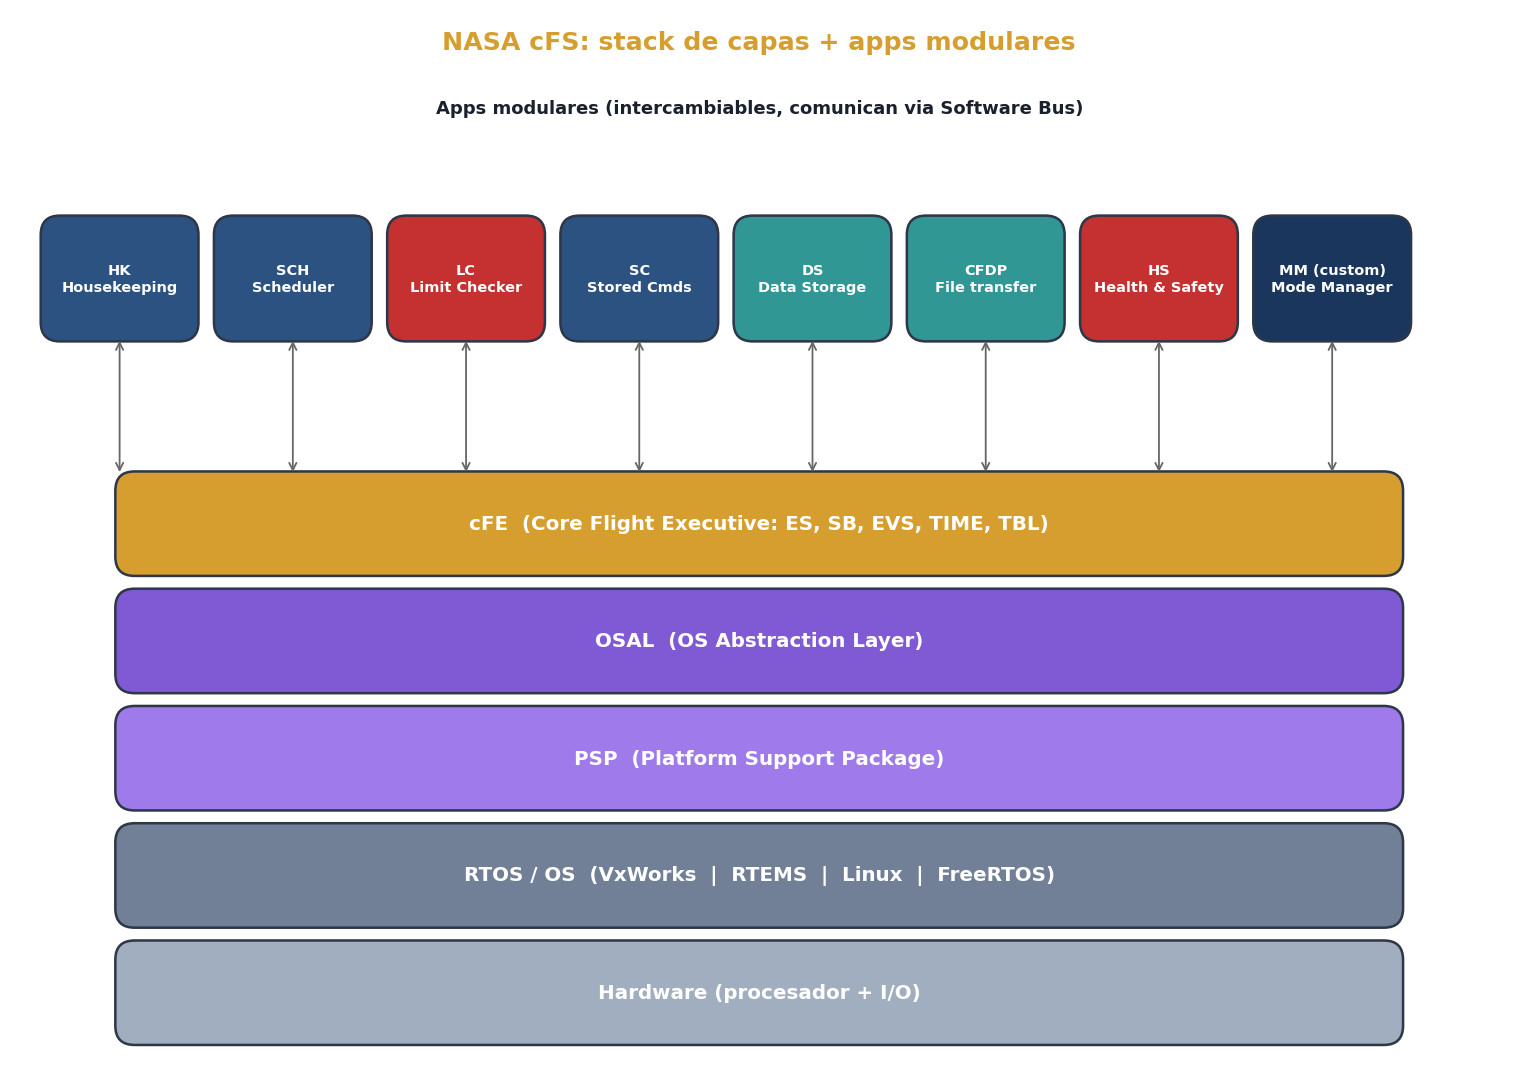
\includegraphics[width=\textwidth]{fig05_cfs.png}
  \caption{Stack de cFS: cuatro capas de plataforma (HW, OS, PSP,
  OSAL) sobre las que corre cFE, y arriba aplicaciones modulares
  intercambiables que comunican por el Software Bus (publish/subscribe).}
  \label{fig:m13-cfs}
\end{figure}

De abajo hacia arriba:

\begin{itemize}[leftmargin=2em]
  \item \textbf{Hardware.} Procesador embebido + perifericos.
  \item \textbf{RTOS/OS.} VxWorks, RTEMS, Linux, FreeRTOS.
  \item \textbf{PSP (Platform Support Package).} Drivers de
    plataforma especificos (board support package).
  \item \textbf{OSAL (OS Abstraction Layer).} Una API uniforme que
    abstrae el RTOS de abajo. Esto permite que la misma aplicacion
    corra sin cambios sobre VxWorks o Linux.
  \item \textbf{cFE (Core Flight Executive).} El runtime real: define
    5 servicios fundamentales descritos abajo.
  \item \textbf{Aplicaciones.} Pluggable, comunican entre si por el
    \emph{Software Bus} de cFE (publish/subscribe).
\end{itemize}

\textbf{Los 5 servicios de cFE.}

\begin{enumerate}[leftmargin=2em]
  \item \textbf{ES (Executive Services).} Lanzar/parar apps, manejar
    tareas y memoria.
  \item \textbf{SB (Software Bus).} Mensajeria publish/subscribe entre
    apps. Es el bus interno del sistema.
  \item \textbf{EVS (Event Services).} Logging estructurado de eventos.
  \item \textbf{TIME.} Reloj del sistema, sincronizado a tiempo de
    mision.
  \item \textbf{TBL (Table Services).} Tablas de parametros
    actualizables desde tierra sin recompilar.
\end{enumerate}

\section{Aplicaciones modulares: el patron clave}

cFS define un \emph{catalogo} de aplicaciones de uso comun que un
equipo puede tomar y meter en su mision:

\begin{itemize}[leftmargin=2em]
  \item \textbf{HK (Housekeeping).} Recolecta telemetria.
  \item \textbf{SCH (Scheduler).} Lanza tareas periodicamente.
  \item \textbf{LC (Limit Checker).} Vigila umbrales (voltajes,
    temperaturas) y dispara alarmas.
  \item \textbf{SC (Stored Commands).} Cola de comandos a ejecutar
    cuando el satelite no esta sobre tierra.
  \item \textbf{DS (Data Storage).} Persistencia de telemetria.
  \item \textbf{CFDP.} Transferencia confiable de archivos (estandar
    CCSDS).
  \item \textbf{HS (Health \& Safety).} Watchdog y modos de seguridad.
\end{itemize}

Cada mision agrega ademas sus \emph{aplicaciones custom}: el manejo
de su payload, su \texttt{MM (Mode Manager)} especifico, drivers de
sus sensores, etc. La clave es que TODO se comunica por el Software
Bus: una app no sabe quien le esta enviando datos, solo se suscribe a
un \emph{message ID}.

\begin{intui}
El gran aporte conceptual de cFS para INTISAT es la separacion
\textbf{Mode Manager como app aparte}. En la mayoria de los CubeSats
estudiantiles, la FSM esta embebida en el ``main'' del firmware. cFS
te obliga a pensarla como una aplicacion separada que escucha eventos
y emite el modo actual al Software Bus. Esto hace mucho mas facil
testearla en aislamiento.
\end{intui}

\section{Que adopta INTISAT y que no}

\begin{logrado}
\textbf{Adoptamos (a nivel conceptual):}
\begin{itemize}[leftmargin=2em]
  \item \textbf{Mode Manager como modulo separado.} En Python tendra
    su propio archivo (\texttt{mode\_manager.py}), no embebido en
    el main loop.
  \item \textbf{Limit Checker explicito.} Un modulo que recorre la
    telemetria y dispara transiciones de modo cuando un umbral se
    cruza.
  \item \textbf{Stored Commands.} Una cola persistente de comandos
    a ejecutar.
  \item \textbf{Pub/sub interno (logico).} En Python lo podemos
    emular con un event bus simple (e.g., \texttt{asyncio.Queue} o
    \texttt{pyzmq}), o incluso una clase con callbacks.
\end{itemize}

\textbf{NO adoptamos:}
\begin{itemize}[leftmargin=2em]
  \item \textbf{cFS en si.} Es C, pensado para RTOS, y portarlo a un
    payload Python sobre Linux es complejidad sin retorno claro
    para una mision 1U.
\end{itemize}
\end{logrado}

\section{Referencias}

\begin{payloadbox}
\textbf{Repo principal.} \url{https://github.com/nasa/cFS}\\[0.3em]
\textbf{Documentacion.}
\url{https://cfs.gsfc.nasa.gov/} (con tutoriales y videos).\\[0.3em]
\textbf{Apps catalog (NASA GitHub).}
\begin{itemize}[leftmargin=2em]
  \item \texttt{nasa/cFE} --- core
  \item \texttt{nasa/osal} --- OS Abstraction Layer
  \item \texttt{nasa/HK}, \texttt{nasa/LC}, \texttt{nasa/SCH},
    \texttt{nasa/SC}, \texttt{nasa/DS}, \texttt{nasa/CFDP},
    \texttt{nasa/HS} --- aplicaciones
\end{itemize}
\textbf{Tutorial recomendado.} La ``cFS 101'' de NASA Goddard
disponible en YouTube; introduce los conceptos en $\sim$2 horas.
\end{payloadbox}

% ============================================================================
\chapter{NASA F' (FPrime)}
% ============================================================================

\section{Que es F' y por que importa}

\textbf{F' (FPrime, pronunciado ``F-prime'')} es un framework de
software de vuelo desarrollado por NASA JPL (Jet Propulsion
Laboratory) y liberado bajo licencia Apache 2.0 en 2017. Es la
respuesta moderna de JPL al problema que cFS resuelve: como construir
software de vuelo modular y reusable. Las diferencias filosoficas con
cFS son significativas.

\textbf{Misiones que lo usaron.}

\begin{itemize}[leftmargin=2em]
  \item \textbf{ASTERIA} (CubeSat 6U, 2017--2020). El primer
    vehiculo en volar F'.
  \item \textbf{MarCO-A y MarCO-B} (mayo 2018). Primeros CubeSats
    interplanetarios; flyby de Marte acompanando a InSight.
  \item \textbf{Ingenuity} (helicoptero en Marte, 2021--2024). 72
    vuelos motorizados en otro planeta; F' coordina todo desde
    sensores hasta motores de rotores.
  \item \textbf{NEA Scout} (2022). Vela solar a un asteroide.
  \item \textbf{LCRD} (2021). Demostracion de comunicacion laser.
\end{itemize}

Que F' haya volado en Marte es la mejor prueba de que el framework
funciona en el peor escenario imaginable: una mision donde el
helicoptero NO puede ser controlado en tiempo real desde la Tierra
(retardo de senal de 5--20 minutos en cada sentido) y donde un bug
imposibilita el vuelo.

\textbf{Lenguaje.} C++ (la unica de nuestras referencias).

\section{Componentes, ports y FPP}

\begin{figure}[h]
  \centering
  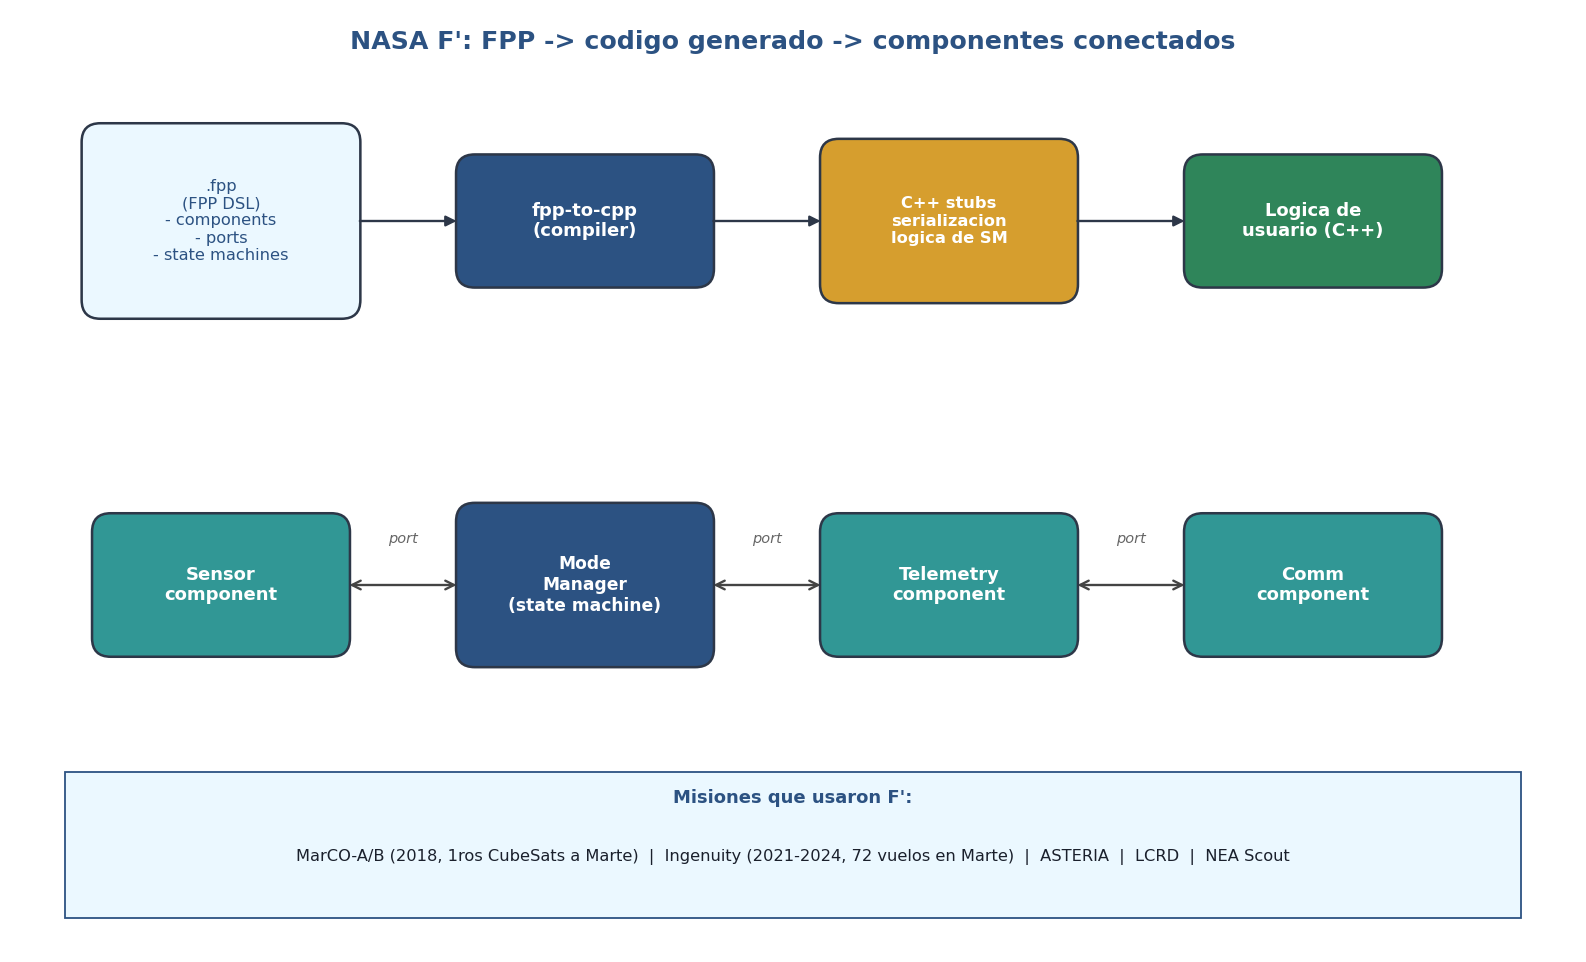
\includegraphics[width=\textwidth]{fig06_fprime.png}
  \caption{Workflow de F': el desarrollador describe su sistema en
  FPP (un DSL), el compilador genera stubs C++, y los componentes
  se conectan via \emph{ports}.}
  \label{fig:m13-fprime}
\end{figure}

\textbf{Conceptos clave.}

\begin{itemize}[leftmargin=2em]
  \item \textbf{Component.} Unidad de funcionalidad. Por ejemplo,
    ``GPS receiver'', ``Camera controller'', ``Mode Manager''. Cada
    component es una clase C++ con estado y metodos.
  \item \textbf{Port.} Interfaz tipada por la que dos components se
    comunican. Es como un metodo, pero el caller no sabe que
    component implementa el callee (loose coupling).
  \item \textbf{Topology.} El \emph{grafo} de quien esta conectado
    con quien. Se describe en un archivo aparte, separado del
    codigo del component.
  \item \textbf{FPP (F Prime Prime).} El DSL textual donde describis
    components, ports, comandos, telemetria, eventos y \emph{state
    machines}. El compilador \texttt{fpp-to-cpp} genera los stubs.
\end{itemize}

\textbf{State machines en FPP.} Aqui esta lo notable: en F' las FSMs
se declaran en FPP y el codigo de las transiciones se genera. El
desarrollador rellena solo las \emph{acciones} de entrada/salida de
estado. Esto reduce los errores tipicos de FSM escritas a mano.

\begin{lstlisting}[style=c, caption=Fragmento estilizado FPP para una FSM de modos]
state machine SatelliteMode {
  initial state Detumbling
  state Detumbling
  state Safe
  state Normal
  state Critical

  transition Detumbling -> Safe on event RatesNominal
  transition Safe -> Normal on event GroundCmd_Activate
  transition Normal -> Critical on event LowBattery
  transition Critical -> Safe on event BatteryRecovered
}
\end{lstlisting}

\textbf{La filosofia es opuesta a cFS}: cFS usa pub/sub (acoplamiento
flojo, runtime-bound), F' usa ports tipados (acoplamiento mediano,
compile-time-bound). Cada uno tiene ventajas en distintos escenarios.

\section{Que adopta INTISAT y que no}

\begin{logrado}
\textbf{Adoptamos (conceptualmente):}
\begin{itemize}[leftmargin=2em]
  \item \textbf{Topologia separada del codigo de cada componente.}
    Aun en Python: la conexion de modulos se describe en un archivo
    de configuracion, no se mezcla con la logica.
  \item \textbf{FSM declarativa.} El \texttt{mode\_manager.py} del
    INTISAT declarara los estados y transiciones como datos
    estructurados, no como \texttt{if/else} dispersos. Esto se
    inspira en F' aunque sin DSL externo.
\end{itemize}

\textbf{NO adoptamos:}
\begin{itemize}[leftmargin=2em]
  \item \textbf{F' framework completo.} C++ es ajeno al equipo y
    el overhead de aprender FPP no se justifica para una mision 1U.
\end{itemize}
\end{logrado}

\section{Referencias}

\begin{payloadbox}
\textbf{Repo principal.} \url{https://github.com/nasa/fprime}\\[0.3em]
\textbf{Documentacion.} \url{https://nasa.github.io/fprime/}\\[0.3em]
\textbf{Misiones que lo usaron.}
\begin{itemize}[leftmargin=2em]
  \item \textbf{Ingenuity Mars Helicopter.} JPL publico un repo
    relacionado: \url{https://github.com/nasa/fprime-tutorial}
  \item \textbf{ASTERIA.} CubeSat de 6U operado en orbita baja
    terrestre entre 2017 y 2020.
\end{itemize}
\textbf{FPP language reference.}
\url{https://nasa.github.io/fpp/}.
\end{payloadbox}

% ============================================================================
\chapter{Sintesis y recomendaciones para INTISAT}
% ============================================================================

\section{Lo que NO debe pasar}

Antes de las recomendaciones positivas, conviene fijar lo que
queremos evitar:

\begin{cuidado}
\begin{enumerate}[leftmargin=2em]
  \item \textbf{Copiar una arquitectura completa que no encaja.}
    Tentacion: ``OreSat es lindo, vamos con CAN+CANopen''. Realidad:
    nuestro equipo no tiene experiencia en CANopen, y para 3
    subsistemas pequenos es over-engineering.
  \item \textbf{Forzar el uso de un framework de NASA.} Tentacion:
    ``si Ingenuity uso F', usemoslo''. Realidad: F' es C++ con un
    DSL externo (FPP) que requiere meses de aprendizaje del equipo.
    INTISAT no tiene ese margen.
  \item \textbf{Saltearse el ``Operations Concept''.} Tentacion:
    ``ya hablamos de los modos, escribimos codigo y vamos viendo''.
    Realidad: AAUSAT y NASA insisten en que el documento de
    operaciones se escriba ANTES del codigo. M12 es ese documento
    para INTISAT.
  \item \textbf{No documentar las decisiones publicamente.} Tentacion:
    ``hagamos issues en un Slack interno''. Realidad: UPSat demostro
    que el Wiki publico de decisiones es lo que permite que el
    equipo siguiente al actual entienda por que estamos haciendo
    lo que hacemos.
\end{enumerate}
\end{cuidado}

\section{Recomendaciones de adopcion selectiva}

\begin{figure}[h]
  \centering
  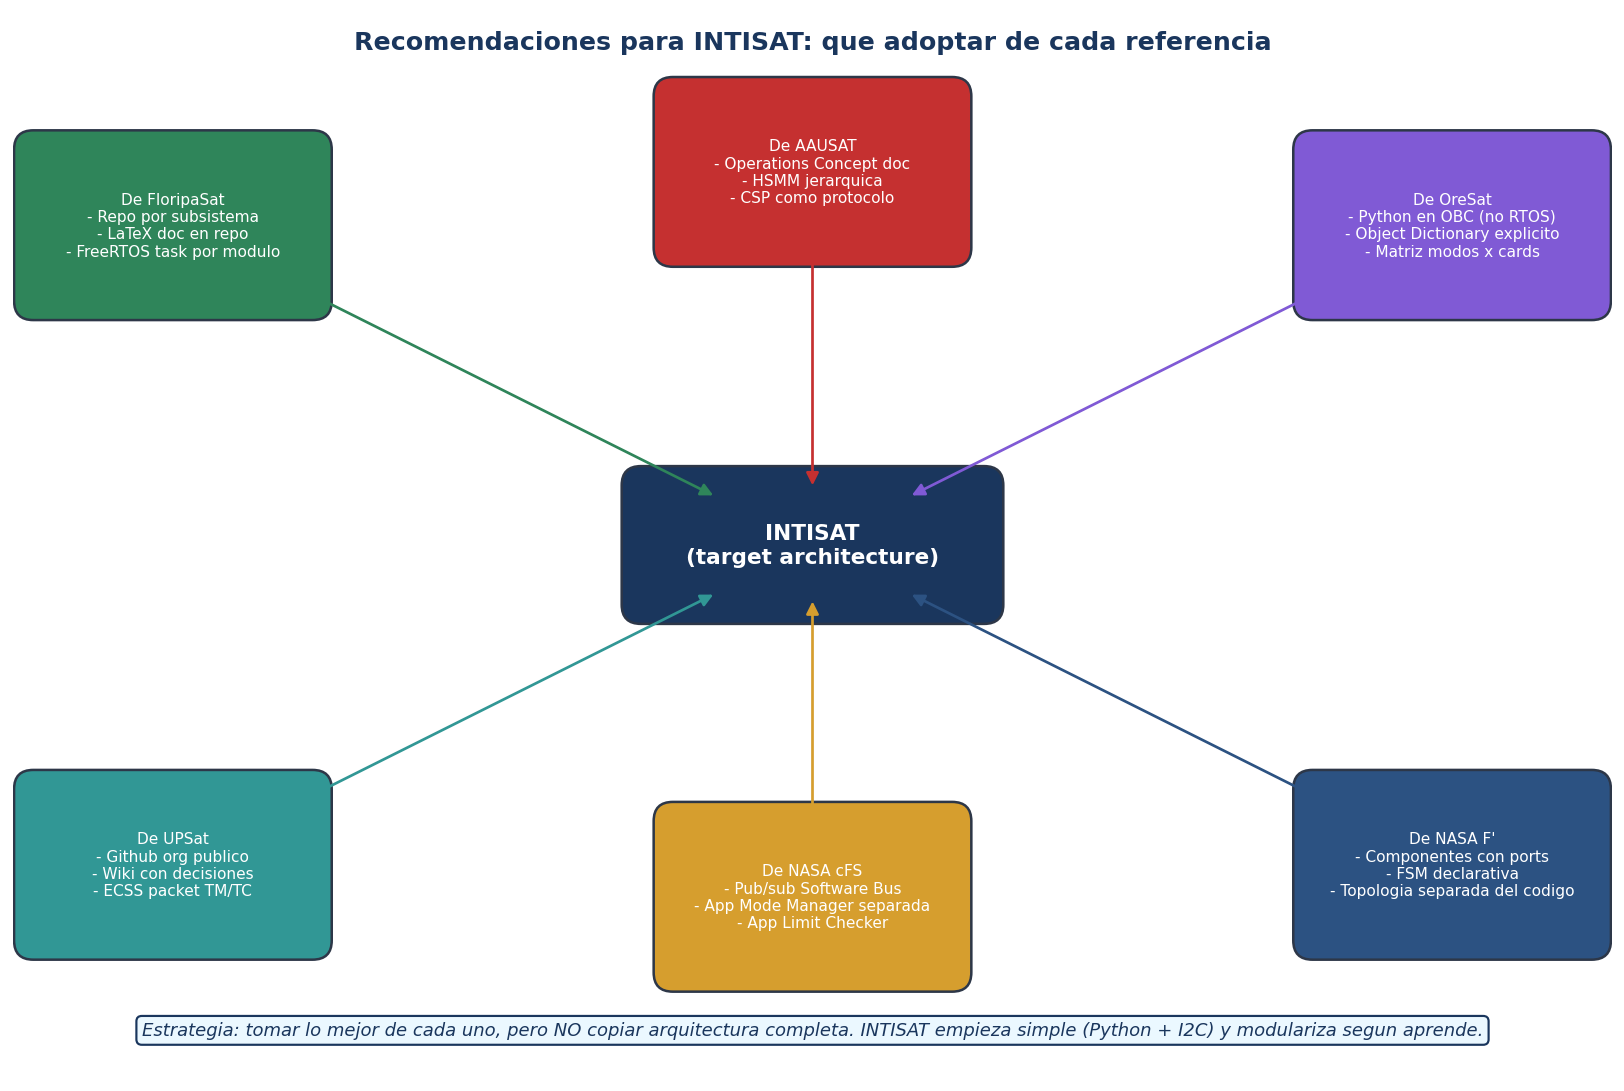
\includegraphics[width=\textwidth]{fig07_recomendacion.png}
  \caption{Sintesis: que toma INTISAT de cada referencia. La estrategia
  es \emph{copiar inteligentemente}, no clonar.}
  \label{fig:m13-recomendaciones}
\end{figure}

\textbf{Resumen por proyecto.}

\begin{enumerate}[leftmargin=2em]
  \item \textbf{De FloripaSat:} repositorio por subsistema +
    documentacion en LaTeX dentro del repo. Beacon como modulo
    independiente del OBDH (es nuestro futuro CubeSat radio).
  \item \textbf{De OreSat:} flight software en Python sobre Linux
    para el OBC, declaracion explicita de telemetria por
    subsistema (Object Dictionary conceptual), modo
    \texttt{PRE\_DEPLOY} con timer obligatorio.
  \item \textbf{De AAUSAT:} el documento ``Operations Concept''
    formal (cumplido por M12), pensar modos como jerarquia (incluso
    si la implementacion inicial es plana), evaluar libcsp para
    una v2 del firmware.
  \item \textbf{De UPSat:} github org publica con Wiki de decisiones,
    aceptar que 4--6 modos en FSM plana es suficiente para 1U,
    paquetes TM/TC con esquema ECSS adaptado.
  \item \textbf{De NASA cFS:} Mode Manager como modulo separado
    (no embebido en el main loop), Limit Checker explicito, Stored
    Commands queue, comunicacion interna pub/sub.
  \item \textbf{De NASA F':} FSM declarada como datos (no
    \texttt{if/else} dispersos), topologia de modulos separada del
    codigo de cada modulo.
\end{enumerate}

\section{Stack final propuesto para INTISAT}

Combinando todo lo anterior, el stack queda:

\begin{tecnico}
\begin{itemize}[leftmargin=2em]
  \item \textbf{OBC:} Raspberry Pi CM5 + Linux (Raspberry Pi OS o
    Yocto custom).
  \item \textbf{Flight software:} Python 3 con \texttt{asyncio} para
    concurrencia. Estructura modular: \texttt{mode\_manager.py},
    \texttt{limit\_checker.py}, \texttt{stored\_cmds.py},
    \texttt{telemetry\_collector.py}, \texttt{payload\_driver.py}.
  \item \textbf{Bus interno:} I2C entre OBC y subsistemas chicos
    (EPS, ADCS, beacon). Cada subsistema chico expone una API
    documentada (analogo conceptual al Object Dictionary de
    CANopen).
  \item \textbf{Telemetria / Telecomando:} paquetes binarios con
    header tipo ECSS (sin todo el overhead del estandar, version
    simplificada). Beacon en AX.25 o FSK directo para radio
    amateur.
  \item \textbf{Documentacion:} esta serie de manuales (M0--M13) en
    LaTeX dentro del mismo repositorio, con figuras generadas
    programaticamente desde \texttt{tools/}.
  \item \textbf{Modos de operacion:} segun M12 (BOOT, SAFE, STANDBY,
    CAPTURA, COMM, CRITICAL).
\end{itemize}
\end{tecnico}

\section{Planilla de decisiones abiertas}

A pesar de toda esta informacion, hay decisiones que el equipo aun
debe tomar antes de cerrar el diseno. Las listamos para que la
proxima reunion las pueda abordar:

\begin{enumerate}[leftmargin=2em]
  \item \textbf{$\zeta$Adoptar libcsp sobre I2C o protocolo ad-hoc?}
    libcsp da rigor de capa de red, pero suma una dependencia C
    importante. Decision en M5.
  \item \textbf{$\zeta$Implementar comandos almacenados (SC)
    desde dia uno o como upgrade post-launch?} Riesgo: si no esta en
    el firmware inicial, no se puede agregar facilmente despues.
  \item \textbf{$\zeta$Usar Yocto o Raspberry Pi OS oficial?} Yocto
    da control fino pero requiere expertise. Raspberry Pi OS arranca
    rapido pero tiene paquetes que no necesitamos.
  \item \textbf{$\zeta$EPS firmware propio o usar uno comercial?}
    GomSpace y Endurosat venden EPS llave-en-mano con CSP. Costo
    vs tiempo de desarrollo.
  \item \textbf{$\zeta$Beacon DIY o modulo comercial?} TT\&C es la
    parte mas regulada y mas critica. Vale la pena no reinventarla.
\end{enumerate}

\section{Cierre}

Construir un CubeSat no es construir un sistema nuevo: es \emph{integrar
decisiones que ya tomaron 50 equipos antes que vos}. Cada uno de los
proyectos que estudiamos en este manual gasto entre 3 y 7 anos de
trabajo de un equipo para responder preguntas que nosotros podemos
contestar leyendo su Wiki. Aprovecharlo no es debilidad: es ingenieria
seria.

Lo unico que hace nuestra mision particular --- el payload de FPM
y la integracion con CM5 --- es donde realmente vamos a aportar algo
nuevo a la comunidad. Todo el resto: arquitectura, modos, telemetria,
ground station, debe ser \emph{lo mas estandar posible} para
liberar tiempo a lo que si nos diferencia.

\begin{logrado}
\textbf{Regla de oro.}
\begin{enumerate}[leftmargin=2em]
  \item Si una decision ya la tomaron $\geq 3$ proyectos de la lista
    y converge a la misma respuesta, ADOPTALA sin discusion.
  \item Si dividieron las respuestas mitad-mitad, ELEGI la mas
    simple para 1U.
  \item Si nadie hizo lo que vos queres hacer, PENSA dos veces por
    que sos el primero. Suele significar que es mala idea o que es
    muy especifica de tu mision.
\end{enumerate}
\end{logrado}

\appendix

% ============================================================================
\chapter{Glosario de terminos}
% ============================================================================

\begin{description}[leftmargin=4em, style=nextline]
  \item[ADCS] Attitude Determination and Control System --- subsistema
    de actitud.
  \item[CAN / CANopen] Bus serie estandar industrial (Bosch, 1986) y
    su capa de aplicacion estandar CiA 301.
  \item[CCSDS] Consultative Committee for Space Data Systems. Cuerpo
    de estandares de comunicacion espacial.
  \item[cFE] Core Flight Executive. El runtime de NASA cFS.
  \item[cFS] Core Flight System. Framework de software de vuelo de
    NASA Goddard.
  \item[CSP] Cubesat Space Protocol. Protocolo de red para CubeSats
    creado en AAUSAT.
  \item[ECSS] European Cooperation for Space Standardization. Cuerpo
    de estandares europeos.
  \item[EDS] Electronic Data Sheet. Archivo de declaracion de Object
    Dictionary en CANopen.
  \item[FPP] F Prime Prime. DSL textual de NASA F'.
  \item[FreeRTOS] RTOS open source, el mas popular en CubeSats.
  \item[FSM] Finite State Machine. Maquina de estados finita.
  \item[HSMM] Hierarchical State Machine Model. FSM con jerarquia
    de modos (statecharts de Harel).
  \item[I2C] Inter-Integrated Circuit. Bus serie 2-hilos de Philips.
  \item[NMT] Network Management. Servicio CANopen para coordinar
    estado de nodos.
  \item[OBDH / OBC] On-Board Data Handling / On-Board Computer. El
    cerebro del satelite.
  \item[OLAF] OreSat Linux App Framework. Framework Python de OreSat.
  \item[OSAL] OS Abstraction Layer. Capa de portabilidad de RTOS.
  \item[PDO] Process Data Object (CANopen). Publicacion periodica
    de telemetria.
  \item[PSP] Platform Support Package (cFS). Drivers de plataforma.
  \item[RTOS] Real-Time Operating System.
  \item[SatNOGS] Red distribuida open-source de estaciones terrenas
    de Libre Space Foundation.
  \item[SDO] Service Data Object (CANopen). Lectura/escritura
    sincronica de objetos.
  \item[SPI] Serial Peripheral Interface. Bus serie 4-hilos.
  \item[TM/TC] Telemetry / Telecommand.
  \item[TT\&C] Telemetry, Tracking and Command. Subsistema de
    comunicaciones.
\end{description}

% ============================================================================
\chapter{Indice de URLs verificables}
% ============================================================================

\section{Misiones universitarias}

\begin{itemize}[leftmargin=2em]
  \item FloripaSat: \url{https://floripasat.ufsc.br/}
  \item FloripaSat GitHub: \url{https://github.com/floripasat}
  \item OreSat: \url{https://www.oresat.org/}
  \item OreSat GitHub: \url{https://github.com/oresat}
  \item AAUSAT: \url{https://www.space.aau.dk/cubesat/}
  \item UPSat (Libre Space): \url{https://libre.space/projects/upsat/}
\end{itemize}

\section{Frameworks NASA}

\begin{itemize}[leftmargin=2em]
  \item NASA cFS GitHub: \url{https://github.com/nasa/cFS}
  \item NASA cFS docs: \url{https://cfs.gsfc.nasa.gov/}
  \item NASA F' GitHub: \url{https://github.com/nasa/fprime}
  \item NASA F' docs: \url{https://nasa.github.io/fprime/}
  \item FPP language: \url{https://nasa.github.io/fpp/}
\end{itemize}

\section{Protocolos y estandares}

\begin{itemize}[leftmargin=2em]
  \item libcsp: \url{https://github.com/libcsp/libcsp}
  \item CANopen CiA 301: \url{https://www.can-cia.org/can-knowledge/canopen/}
  \item CCSDS estandares: \url{https://public.ccsds.org/Publications/}
  \item ECSS estandares: \url{https://ecss.nl/}
\end{itemize}

\section{Infraestructura terrestre open}

\begin{itemize}[leftmargin=2em]
  \item SatNOGS: \url{https://satnogs.org/}
  \item Libre Space Foundation: \url{https://libre.space/}
  \item GNU Radio: \url{https://www.gnuradio.org/}
\end{itemize}

\end{document}
